%This is the Preface
%%=========================================
\addcontentsline{toc}{section}{Abstract}
\begin{center}
\section*{Abstract}
\end{center}

Internet of Things (IoT) applications very often involve the use of sensors. Motion sensing can be used in a vast amount of applications and are therefore very interesting in high volume IoT products. Replacing a battery in such applications is often undesirable, and may in some cases be close to impossible. It is therefore essential for such products to have sensors that consumes as little power as possible. 

This specialization project presents a thorough analysis of five commercially available microelectromechanical (MEMS) accelerometers. The analysis focuses primarily on finding the sensor that is best suited for a broad range of ultra low power IoT applications. The best sensor is chosen to be a part of a custom reference board, of which also was designed as a part of this work. The reference board is planned to be used for a later Master thesis, where the goal is to further explore different IoT application areas for ultra low power motion sensors.

From the analysis in this work it has been showed that the ADXL362 from Analog Devices currently is the most low power accelerometer available on the market. The same device is also quite versatile, with many different configuration options, which makes it perfectly suited for a broad range of IoT applications. Some of the most relevant are simple motion detection, vibration detection and inertial navigation.  

The project is carried out as feasibility analysis for Disruptive Technologies AS in conjunction with the Norwegian University of Science and Technology (NTNU).

\begin{center}
Trondheim, 2015-20-12\\[1pc]
\begin{figure}[h]
\centering
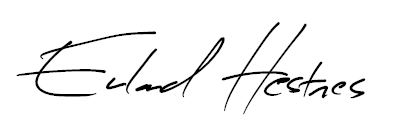
\includegraphics[scale=0.5]{fig/underskrift.png}
\label{fig:underskrift}
\end{figure}
Erlend Hestnes
\end{center}